\documentclass[11pt]{article}
\usepackage[a4paper,margin=1in]{geometry}
\usepackage[T1]{fontenc}
\usepackage[utf8]{inputenc}
\usepackage{amsmath,amssymb,amsfonts,mathtools}
\usepackage{booktabs}
\usepackage{array}
\usepackage{adjustbox}
\usepackage{enumitem}
\usepackage{float}
\usepackage[table]{xcolor}
\usepackage{listings}
\usepackage{longtable}
\usepackage{tikz}
\usepackage{hyperref}
\usetikzlibrary{arrows.meta,positioning}

% --- Mathematica lstlisting style ---
\definecolor{listinggray}{rgb}{0.5, 0.5, 0.5}
\definecolor{listinggrayer}{rgb}{0.95, 0.95, 0.95}
\definecolor{mmacomment}{rgb}{0.35,0.35,0.35}
\definecolor{mmastring}{rgb}{0.6,0.1,0.1}
\lstdefinestyle{MathematicaStyle}{
    language=Mathematica,
    breaklines=true,
    breakatwhitespace=false,
    breakindent=1em,
    basicstyle=\ttfamily\small,
    columns=flexible,
    linewidth=0.92\linewidth,
    frame=single,
    showstringspaces=false,
    numbers=left,
    numberstyle=\tiny\color{listinggray},
    backgroundcolor=\color{listinggrayer},
    commentstyle=\color{mmacomment}\itshape,
    stringstyle=\color{mmastring},
    literate={+}{+}{1} {a}{a}{1} {b}{b}{1} {c}{c}{1} {d}{d}{1} {e}{e}{1} {f}{f}{1} {g}{g}{1} {h}{h}{1} {i}{i}{1} {j}{j}{1} {k}{k}{1} {l}{l}{1} {m}{m}{1} {n}{n}{1} {o}{o}{1} {p}{p}{1} {q}{q}{1} {r}{r}{1} {s}{s}{1} {t}{t}{1} {u}{u}{1} {v}{v}{1} {w}{w}{1} {x}{x}{1} {y}{y}{1} {z}{z}{1} {A}{A}{1} {B}{B}{1} {C}{C}{1} {D}{D}{1} {E}{E}{1} {F}{F}{1} {G}{G}{1} {H}{H}{1} {I}{I}{1} {J}{J}{1} {K}{K}{1} {L}{L}{1} {M}{M}{1} {N}{N}{1} {O}{O}{1} {P}{P}{1} {Q}{Q}{1} {R}{R}{1} {S}{S}{1} {T}{T}{1} {U}{U}{1} {V}{V}{1} {W}{W}{1} {X}{X}{1} {Y}{Y}{1} {Z}{Z}{1} {0}{0}{1} {1}{1}{1} {2}{2}{1} {3}{3}{1} {4}{4}{1} {5}{5}{1} {6}{6}{1} {7}{7}{1} {8}{8}{1} {9}{9}{1} {\}}{\}}{1},
    xleftmargin=1em,
    xrightmargin=1em
}

\lstdefinestyle{MathematicaOutput}{
    basicstyle=\ttfamily\small,
    columns=flexible,
    linewidth=0.92\linewidth,
    frame=single,
    rulecolor=\color{listinggray},
    showstringspaces=false,
    numbers=none,
    backgroundcolor=\color{white},
    xleftmargin=1em,
    xrightmargin=1em
}

% --- Macros ---
\newcommand{\U}{\mathcal{U}_n}
\newcommand{\bits}{\{0,1\}}

\title{Causal Compression of Boolean Networks via Algorithmic Querying}
\author{Alberto Hern\'andez-Espinosa \and Hector Zenil}
\date{}

\begin{document}
\maketitle

\begin{abstract}
We study the patterns that deterministic Boolean networks imprint across
their exhaustive input--output repertoires.  Gate rules, acting on a fixed
connectivity structure, distribute information through the configuration
space in a manner that is neither random nor immediately transparent: the
resulting output sequences appear complex, yet conceal regularities that
can be captured by short generative descriptions.
We formalise this observation into a causal compression methodology situated
in the exactly solvable limit of Algorithmic Information Dynamics---the
regime in which the generating mechanism is given, so that the shortest
description in a declared language may be computed rather than estimated---and
grounded in the Principle of Computational Equivalence.
For each of the twelve canonical Boolean gate families---monotone, parity,
threshold, implication, negation, and canalising---we derive exact
compressed representations and a deconvolution process that recovers the
complete one-set of any gate without row-wise evaluation.
We demonstrate compression first for isolated gates, then for multi-node
queries where several gates are interrogated simultaneously, and finally
for the full system, showing that the effective search space compresses
by exact factors that depend on the interaction structure rather than
the network size.
Because the exact generating programme and its exact description length are
both available here, these networks serve as a calibration class for methods
that must operate without such knowledge: we measure a block-decomposition
estimator against ground truth and find it within a factor of $4.3$ of the
true programme length, while statistical baselines on the same object remain
two orders of magnitude away.
These results demonstrate that the full complexity of a Boolean network's
behaviour is generated by short causal rules that can be identified,
formalised, and exploited computationally.
\end{abstract}


%%% ===========================================================================
\section{Introduction}\label{sec:intro}
%%% ===========================================================================

Boolean networks are deterministic dynamical systems,
yet they exhibit the full phenomenology that makes complex systems
singular: sensitive dependence on initial conditions,
attractor multiplicity, and the exponential growth of the configuration
space with system size.  Since Kauffman's pioneering
work~\cite{kauffman}, they have served as objects of study in
theoretical biology, gene regulation, and the broader investigation of
how simple local rules generate complex collective
behaviour~\cite{wolfram2002new}.

Two fundamental questions pervade the analysis of such systems. First, 
what are the mechanisms by which order emerges in deterministic networks? 
Second, in what sense do global dynamics exhibit emergent properties that 
are not reducible to local update rules? These questions can be 
technically instantiated within Boolean networks, where each node 
applies a deterministic local rule and the full system behaviour is, 
in principle, computable. The difficulty is not computational power; 
it is \emph{causal compression}. One can always enumerate a truth table 
or run a simulation. What remains elusive is a representation that is at 
once exact, compositional, and explanatory---one that identifies the 
generative rule structure responsible for the observed outputs rather 
than merely reproducing 
them~\cite{kauffman1993origins,wolfram2002new,clarke2019compositional,li2011dynamics}.

This paper presents a causal compression methodology for Boolean networks
that is grounded in two intellectual traditions.  The first is the
Principle of Computational Equivalence (PCE)~\cite{wolfram2002new}, which
holds that simple discrete rules generate the full complexity observed in
natural and computational systems.  The second is Algorithmic Information
Dynamics (AID)~\cite{zenilcalculus,zenildeconv,zenilaidbook}, which provides an
inferential and interventionist calculus for recovering short generative
rules from observations, emphasising algorithmic probability, generative
mechanisms, and causation over surface statistics.

Our relation to AID is best stated precisely, since it determines what may
and may not be claimed here.  AID in its general form addresses an inverse
problem under uncertainty: the generating mechanism is unknown, and one
estimates algorithmic content by perturbation and approximation of
algorithmic probability.  The present work occupies the corner of that
programme in which the mechanism is \emph{given}.  A Boolean network is a
controlled object---its wiring and its gates are known---so no estimation
is required on the mechanism side, and the shortest description in a
declared language can be written in closed form rather than approximated.
We therefore present this method not as an alternative to AID but as its
\emph{exactly solvable limit}: the regime in which the quantities that AID
must estimate can instead be computed.  What we contribute back to AID is
correspondingly specific---not a new estimator, but a class of objects with
known exact generating programmes and known description lengths, against
which estimators can be calibrated.  We exercise that calibration in
Section~\ref{sec:description-length}.

The currency of the argument follows from this position.  A description is
taken to be explanatory when it is a programme that reproduces the observed
behaviour exactly, and its cost is measured by the length of that programme
rather than by the entropy of the behaviour it produces.  This is the sense
in which compression stands in for comprehension~\cite{zenilcomprehension}:
a short programme that regenerates a large object constitutes an account of
that object, whereas an entropy figure quantifies a coding cost and
explains nothing.  The distinction is not rhetorical here but measurable,
and Section~\ref{sec:description-length} reports the measurement.

Our analysis is based on the observation that when the
output of a Boolean network is examined node by node across the
ordered exhaustive repertoire, the isolated output sequences are not
random: they exhibit self-similar patterns replicated at several scales.  The
resulting information distribution---what was termed ``fractal behaviour''
in earlier work~\cite{hernandez2019}---is a structural consequence of the
interaction between the network topology and the deterministic local
rules.

The key insight is that this self-similar structure admits exact
compressed representations.  For any Boolean gate operating within a
network of $n$ nodes, the complete set of repertoire indices at which
the gate outputs one can be expressed as two short objects: a \emph{base
set} $L$ of decimal anchors, and an \emph{offset family} $\Omega$.
Deconvolution of this pair---adding each sumando to each decimal anchor---recovers
the exact one-set without evaluating a single row.  The base set
encodes the gate semantics; the offset family encodes the network
topology.  Together, they constitute a short generative programme whose
output is the full behaviour of the gate across $2^n$ input states.

The self-similarity is not a metaphor but a property of $\Omega$, and it can
be stated mechanically.  Each coordinate that does not feed the node
contributes an independent binary choice, so $\Omega$ factorises as a sumset
of powers of two, $\bigoplus_j\{0,2^{\,j-1}\}$ over the free coordinates.  The
activation pattern therefore recurs at every partial sum of those weights,
which is dyadic rescaling in a literal sense: the same short pattern, laid
down at geometrically spaced intervals across the repertoire.  This is what
was observed informally as ``fractal'' behaviour, and it is exactly why a
description of the pair $(L,\Omega)$ suffices where a listing of the sequence
does not.

In this paper we treat twelve families: AND, OR, XOR, NAND, NOR, XNOR, NOT, IMPLIES,
NIMPLIES, KOFN (threshold), MAJORITY, and CANALISING, which exhaust the
standard gate catalogue used in Boolean network modelling.

We compare experiments with networks of different sizes to show that 
the compression factor is independent of the network size and we 
confirm that analytic evaluation time does not grow with the ambient
dimension~$n$---it is governed by the support-union instead, and stays of the
order of a millisecond or below across the whole range tested.

The perspective is \emph{causality-first} in three senses.  First, it is
rule-first rather than correlation-first: the object of study is the
generative logic of the system, not its observed frequencies.
Second, it is deterministic rather than statistical: the method
reconstructs exact behaviour under known dynamics, not approximate
inference under unknown mechanisms.  Third, it is compositional: global
behaviour is built from local causal rules, and the compression reflects
the causal structure of the mechanism itself.
All computational experiments are reproducible via the companion code
repository (see Appendix~\ref{app:code}).


%%% ===========================================================================
\section{Background}\label{sec:background}
%%% ===========================================================================

\subsection{Boolean networks and ordered repertoires}\label{sec:bn-setup}

A Boolean network of size $n$ is specified by a connectivity matrix
$cm\in\bits^{n\times n}$, where $cm_{ij}=1$ means node $j$ feeds node $i$,
and a dynamic vector $\mathit{dyn}=(d_1,\ldots,d_n)$ listing the local
Boolean gate at each node (see lines 1-11 in Listing code~\ref{6-nodes-list-code}). 

The connected-input set of node $i$ is
$N_i=\{j:cm_{ij}=1\}$, and the synchronous one-step update is
\[
F(x)=\bigl(g_1(x_{N_1}),\ldots,g_n(x_{N_n})\bigr),
\qquad x\in\bits^n.
\]
where $x$ represents an input vector in the input repertoire that composes
an \emph{ordered exhaustive repertoire} that is the set of all $2^n$ input
vectors under a declared enumeration.  
Throughout this paper we use
LSB-first ordering, in which the $j$-th vector is
$v(j)=\mathrm{Reverse}(\mathrm{IntegerDigits}(j{-}1,2,n))$ with bit
weights $w(i)=2^{i-1}$.  The resulting index universe is
$\mathcal{U}_n=\{1,\ldots,2^n\}$.

\subsection{Gate families and output signatures}\label{sec:gate-families}

When the output of a single node is isolated across the ordered
exhaustive repertoire, the resulting binary sequence, this is, a string of ones
and zeros of length $2^n$, reveals patterns characteristic of the gate
that node implements.  These patterns are the starting point of the
method: before any formal derivation, one observes the regularities in
the output sequences that each gate family produces when embedded in a
network.

The observation is most transparent for a small case examined in full.
Consider the seven-node network of Listing~\ref{7-nodes-list-code}, and
within it node~4: an AND gate reading inputs $\{1,3,5,7\}$.

\begin{lstlisting}[style=MathematicaStyle,caption={Seven-node network used
throughout this section.  Node 4 is an AND gate over inputs $\{1,3,5,7\}$;
nodes $\{2,4,6\}$ do not feed it.},label={7-nodes-list-code}]
cm07 = {{0, 0, 1, 0, 0, 0, 1},
        {0, 0, 1, 0, 0, 1, 0},
        {1, 0, 0, 0, 1, 0, 1},
        {1, 0, 1, 0, 1, 0, 1},
        {0, 0, 1, 1, 0, 1, 1},
        {1, 1, 1, 0, 0, 0, 0},
        {0, 1, 0, 1, 1, 1, 0}};
dyn07 = {"AND", "OR", "OR", "AND", "OR", "OR", "AND"};
\end{lstlisting}

Isolating node~4 across the ordered exhaustive repertoire gives a
$128$-element binary string.  It is dominated by zeros, since an AND gate
fires only when \emph{all} connected inputs are simultaneously active.
Written out in full, with the eight firing positions marked, the string is

\begin{lstlisting}[style=MathematicaOutput]
positions   0 ................................................... 84   (all 0)
positions  85  86  87  88 ... 92  93  94  95  96 ............... 116
             1   0   1   0        1   0   1   0                        (0)
positions 117 118 119 120 ... 124 125 126 127
             1   0   1   0         1   0   1
\end{lstlisting}

\noindent
so the gate outputs one exactly at positions
$\{85,87,93,95,117,119,125,127\}$, using $0$-based repertoire indices.

A flat run-length encoding of this string reads
$\{85 \!\to\! 0,\; 1 \!\to\! 1,\; 1 \!\to\! 0,\; 1 \!\to\! 1,\;
5 \!\to\! 0,\; 1 \!\to\! 1,\; 1 \!\to\! 0,\; 1 \!\to\! 1,\;
21 \!\to\! 0,\; \ldots\}$, where each pair $k \!\to\! v$ denotes $k$
consecutive occurrences of digit~$v$.  Sixteen such runs, thirty-two
tokens, describe the sequence completely.

That encoding is nevertheless the wrong object, and it is worth saying why
plainly, because the distinction is the whole point of the method.  A
run-length listing is a \emph{tally}: it records the sequence faithfully and
generates nothing.  It offers no account of why the gaps between firings have
lengths $1$, $5$ and $21$ rather than any other lengths, and it would grow
without bound as $n$ grows.  What the method seeks is the rule that produces
those gaps.

That rule is exact and short.  The four connected inputs carry bit weights
$1+4+16+64=85$, and an AND gate fires only when all four are set, which fixes
a single decimal anchor: the base set is $L=\{85\}$.  The three disconnected
coordinates $\{2,4,6\}$ carry weights $\{2,8,32\}$ and are free to take any
values, so the offset family is the set of all their subset sums.  Crucially,
that family \emph{factorises}, one independent binary choice per free
coordinate:
\[
\Omega \;=\; \{0,2\}\oplus\{0,8\}\oplus\{0,32\}
\;=\;\{0,2,8,10,32,34,40,42\},
\]
where $\oplus$ denotes the sumset $A\oplus B=\{a+b\}$.  Deconvolution
recovers the firing positions exactly:
\[
\operatorname{Dec}(L,\Omega)=\{85,87,93,95,117,119,125,127\}.
\]

Two features of this description deserve emphasis.  First, it is
\emph{nested} rather than sequential: the activation pattern is stated once
and recurs at every partial sum of the free weights, which is exactly why the
sequence appears self-similar at dyadic scales, and exactly what the flat
tally destroys.  The gap lengths $1$, $5$ and $21$ are not primitive data but
consequences of the weights $2$, $8$ and $32$.  Second, it is dramatically
shorter: one decimal anchor and three free weights---four numbers---against
thirty-two run-length tokens, and the gap widens as $n$ grows because $L$ and
$\Omega$ depend on the node's support rather than on the size of the
repertoire.  Every figure in this example is regenerated by the companion
script \texttt{worked\_example\_7node.py}.

An OR gate produces the complementary picture: long runs of ones
interrupted by rare clusters of zeros, since the gate fires whenever
\emph{any} input is active.  XOR and XNOR gates yield periodic
alternation governed by the parity of active inputs.  Threshold gates
(KOFN, MAJORITY) produce layered transitions whose boundaries correspond
to Hamming-weight levels.  Implication and canalising gates exhibit
asymmetric signatures reflecting the privileged role of specific inputs.

\paragraph{The representation is a schema normal form.}
The structure just exhibited has a precise name.  A \emph{schema} in
Holland's sense~\cite{holland1975} is a template over $\{0,1,*\}$, in which
$*$ marks a position whose value does not affect membership.  The worked
example is exactly such a template: node~4 fires on the schema
$1\,\ast\,1\,\ast\,1\,\ast\,1$ read over coordinates $1$ to $7$, with its four
connected inputs $\{1,3,5,7\}$ fixed at one and the three disconnected
coordinates $\{2,4,6\}$ free.  This is not an analogy.  For every gate family in
Table~\ref{tab:gate-families}, the one-set is precisely a union of schemata,
and the pair $(L,\Omega)$ is a normal form for that union: $L$ enumerates
the determined coordinates, $\Omega$ enumerates the fillings of the
don't-care positions.  Deconvolution is the instantiation of the template.

The correspondence is quantitative as well as structural.  The \emph{order}
of a schema---its number of fixed positions---is exactly the support size
$|C_q|$ of the corresponding query, and the count of don't-care positions is
$n-|C_q|$, whence $|\Omega|=2^{\,n-|C_q|}$.  The scalability result reported
in Section~\ref{sec:benchmarks}, that analytic cost is governed by $|C_q|$
rather than by $n$, is therefore a statement about schema order: low-order
schemata are cheap to evaluate however large the ambient space becomes.

\paragraph{What the disconnected coordinates do.}
It is worth being exact about the role of the coordinates that do not feed a
node, because the natural summary---that they are irrelevant---is true at
only one of three levels.

\begin{itemize}[leftmargin=1.4em]
\item \emph{Per node, per step.} They do not affect the output \emph{value}.
  This is precisely what makes them don't-care positions, and it is why the
  gate semantics can be read off from $L$ alone.
\item \emph{Per repertoire.} They nevertheless determine \emph{where} and
  \emph{how often} the activation pattern occurs: their bit weights generate
  $\Omega$, fixing its cardinality $2^{\,n-|C_q|}$ and the dyadic spacing at
  which the pattern recurs.  They are causally inert as to the value and
  constitutive of the structure of the behaviour.
\item \emph{Per query.} Membership of the don't-care set is not intrinsic to
  a node.  When several nodes are interrogated jointly, the free set is
  recomputed against the \emph{union} of their supports, so a coordinate that
  is a don't-care for one node ceases to be one as soon as a co-queried node
  reads it.  The amount by which the free set contracts is the overlap
  $\mu_q$ of Section~\ref{sec:overlap}, and the resulting factor $2^{\mu_q}$
  is what makes joint queries cheaper than the product of separate ones.
\end{itemize}

\noindent
The third level is where interaction enters.  Don't-care status is a property
of the query, not of the network, and integration is measured by exactly how
much it shrinks under joint interrogation.  We note that this concerns the
geometry of the one-set under one synchronous step; over several steps a
coordinate outside $C_q$ may of course become an ancestor of the node, which
is a separate question.

Two observational tools proved essential for identifying these
regularities.  First, \emph{run-length encoding} compresses each output
sequence into a short list of $(k \!\to\! v)$ pairs, making the
repetitive structure visible---though, as the worked example showed, it
records rather than generates.  Second, schemata identify which input
coordinates determine the output and which are free to vary.  Together,
these tools revealed that every gate family produces output sequences whose
structure can be described by a short generative rule, and that the formal
characterisation of each family follows from formalising these observed
patterns.

Table~\ref{tab:gate-families} summarises the formal one-set
structure---the set of repertoire indices at which each gate outputs
one---that emerges from this pattern analysis, expressed in terms of
coordinate bands, parity classes, and Hamming-weight layers.

\begin{table}[h]
\centering
\small
\begin{tabular}{@{}lp{0.62\linewidth}@{}}
\toprule
\textbf{Gate family} & \textbf{One-set structure} \\
\midrule
AND      & Intersection of one-bands of all connected inputs \\
OR       & Union of one-bands \\
NAND     & Complement of AND one-set \\
NOR      & Intersection of zero-bands (complement of OR) \\
XOR      & Odd-parity class over connected inputs \\
XNOR     & Even-parity class \\
NOT      & Zero-band of the single connected input \\
IMPLIES  & Complement of (antecedent one-band $\cap$ consequent zero-band) \\
NIMPLIES & Antecedent one-band $\cap$ consequent zero-band \\
KOFN     & Union of Hamming-weight layers at or above threshold $k$ \\
MAJORITY & KOFN with $k=\lceil d/2 \rceil$ \\
CANALISING & Trigger set $\cup$ (non-trigger $\cap$ fallback one-set) \\
\bottomrule
\end{tabular}
\caption{Formal one-set structure for each gate family, derived from the
observed output patterns.  Band $\mathcal{B}_i^a$ denotes the set of
indices where coordinate $i$ equals $a$; parity and weight classes are
defined analogously.  Full derivations appear in~\cite{formalmanuscript}.}
\label{tab:gate-families}
\end{table}

The key observation is that \emph{all} of these one-sets share a common
structural property: each decomposes into a short activation pattern that
encodes the gate semantics, replicated across the repertoire by shifts
that encode the network topology.  This universal decomposition is what
makes compressed representation possible across the full gate catalogue.

\subsection{Self-similar patterns and compressed representation}\label{sec:decomposition}

The patterns described above are not merely compact descriptions of
individual outputs; they reveal a deeper structural regularity.  When
the output of a single node is examined across the ordered exhaustive
repertoire, the same activation sub-pattern recurs at geometrically
spaced intervals throughout the sequence.  This self-similar
structure---what was termed ``fractal behaviour'' in earlier
work~\cite{hernandez2019}---is not an artefact of any particular gate
type but a general property of deterministic Boolean networks operating
on binary-encoded input spaces.

The discovery followed a natural path.  The perturbation test---evaluating
the network on every possible input---produces for each node an output
sequence of length $2^n$.  Examined in isolation, these sequences appear
complex: for a seven-node network, the output of any given node is a
128-element binary string with no immediately obvious rule.  Yet when
described using run-length notation and schemata, the same short
sub-pattern is found to replicate across the sequence at intervals that
follow a geometric progression tied to powers of two.

This observation admits a precise representation as two short objects:

\begin{itemize}
\item The \textbf{base set} $L$ (termed \emph{DecimalRepertoire} in the
  companion code): the repertoire indices at which the node outputs one
  when only its connected inputs vary and all other coordinates are held
  at zero.  This set captures the gate's intrinsic activation rule as it
  operates within the network.
\item The \textbf{offset family} $\Omega$ (termed \emph{Sumandos}): the
  set of shifts at which the base-set pattern is replicated across the
  full repertoire.  Each shift corresponds to an assignment of the
  remaining coordinates---those that do not feed the node---and the
  geometric spacing of these shifts is what produces the self-similar
  structure observed in the output sequences.
\end{itemize}

The full one-set is recovered by \emph{deconvolution}:
\[
\mathcal{J} = \operatorname{Dec}(L,\Omega)
= \{\ell + \omega : \ell\in L,\; \omega\in\Omega\}.
\]
This operation unfolds the compressed pair into the exact set of
repertoire positions at which the node outputs one, without evaluating a
single row of the truth table.  The base set encodes the short rule that
the gate produces; the offset family encodes where that rule repeats.

The mathematical explanation for this decomposition is straightforward:
the connected inputs determine the gate's activation condition, while the
disconnected inputs---those coordinates absent from the node's row in the
connectivity matrix---are free to take any value without affecting the
output.  Their bit weights generate the offset family as a sumset of
powers of two.  But the method was not derived from this algebraic
observation.  It was discovered by inspecting the output sequences,
identifying their self-similar structure, and then recognising that the
structure could be expressed as a short generative rule.  The
connected/disconnected decomposition is the mathematical explanation of
\emph{why} the patterns exist; the patterns themselves are what the method
observes and exploits.

\subsection{Causal querying and algorithmic complexity}\label{sec:aid-querying}

Within the AID framework~\cite{zenilcalculus,zenildeconv}, the compressed
representation constitutes a short generative programme for the gate's
behaviour, and the deconvolution is its execution.  The methodology is a
form of causal querying: given a known deterministic mechanism (the Boolean
network), one asks which input conditions produce a specified output event,
and the answer takes the form of a programme that is dramatically shorter
than the output it generates.

The object described is accordingly individual rather than
ensemble~\cite{hernandez2019}.  Methods built on regression, correlation or
probability distributions---transfer entropy, Granger causality, partial
information decomposition---characterise the family of sequences a source
emits.  The base set and offset family instead describe this network's
input--output map and no other.  Section~\ref{sec:description-length} makes
the consequence quantitative.

This connects to the perturbation asymmetry central to
AID~\cite{zenilcalculus}.  An algorithmically simple object---one
generated by a short programme---is sensitive to perturbation: modifying
the programme propagates non-linearly through the output.  A random
object is insensitive: its shortest description is the object itself.
The compressed representation of a Boolean network is exactly such a
short programme, and its brevity relative to the full output table is a
quantitative signature of the causal structure of the mechanism.


%%% ===========================================================================
\section{Causal Querying and Compressed Representations}\label{sec:querying}
%%% ===========================================================================

All code listings in this section and the next use two core functions from
the companion library (see Appendix~\ref{app:code}):
\texttt{ApplyGate[gate, inputs, params]} evaluates a single Boolean gate
on a given input vector, and
\texttt{CreateRepertoiresDispatch[cm, dyn, params]} builds the full
$2^n$-row exhaustive repertoire by applying \texttt{ApplyGate} to every
row of the ordered input space.

\subsection{Single-gate case: AND deconvolution}\label{sec:and-deconv}

We begin with the simplest non-trivial case: a single AND gate inside a
six-node network.

\begin{lstlisting}[style=MathematicaStyle,caption={Six-node network definition and exhaustive repertoire via gate dispatch.},label={6-nodes-list-code}]
(* Load companion library *)

cm06 = {
  {1, 0, 0, 0, 0, 0},
  {0, 1, 0, 0, 0, 0},
  {0, 0, 1, 0, 0, 0},
  {1, 0, 0, 1, 0, 0},
  {0, 1, 0, 1, 0, 0},
  {1, 0, 1, 0, 1, 0}
};
dyn06 = {"OR","NOT","OR","IMPLIES","AND","XOR"};

dispatch06 = CreateRepertoiresDispatch[cm06, dyn06];
inputs06  = dispatch06["RepertoireInputs"];
outputs06 = dispatch06["RepertoireOutputs"];

Length[inputs06] = 64
inputs06[[1;;3]]  = {{0,0,0,0,0,0},{1,0,0,0,0,0},{0,1,0,0,0,0}}
outputs06[[1;;3]] = {{0,1,0,1,0,0},{1,1,0,0,0,1},{0,0,0,1,0,0}}
\end{lstlisting}


Node~5 is an AND gate with connected-input set $N_5=\{2,4\}$, extracted
directly from the connectivity matrix.
The network has $n=6$, so the exhaustive repertoire contains $2^6=64$ rows.
The question is: at which of these 64 rows does node~5 output one?

The compressed representation answers this without evaluating any row.
Under LSB-first ordering, the bit weights are $w(i)=2^{i-1}$, so the
connected contribution (the \emph{decimal anchor}) is
$P(N_5) = w(2)+w(4) = 2+8 = 10$.
The disconnected inputs are $\{1,3,5,6\}$, and their offset family is the
set of all sums of subsets of the corresponding weights:

\begin{lstlisting}[style=MathematicaStyle,caption={Computing the offset family and AND deconvolution.}]
weights[n_] := 2^Range[0, n - 1];

allOffsets[n_, connected_] := Module[
  {free = Complement[Range[n], connected], ws},
  ws = weights[n][[free]];
  Sort[(# . ws) & /@ Tuples[{0, 1}, Length[ws]]]
];

givePlaces[locations_, sumandos_] :=
  Sort@Flatten[Table[loc + sumandos, {loc, locations}]];

ic5 = Sort@Flatten@Position[cm06[[5]], 1]
decimalAnchor5 = 1 + Total[weights[6][[ic5]]]
offsets5 = allOffsets[6, ic5]
predicted5 = givePlaces[{decimalAnchor5}, offsets5]
\end{lstlisting}
\begin{lstlisting}[style=MathematicaOutput]
(* ic5      = {2, 4}                                                *)
(* decimalAnchor5   = 11                                                    *)
(* offsets5 = {0,1,4,5,16,17,20,21,32,33,36,37,48,49,52,53}        *)
(* predicted5 = {11,12,15,16,27,28,31,32,43,44,47,48,59,60,63,64}  *)
\end{lstlisting}

Corroboration against the exhaustive baseline produced by
\texttt{CreateRepertoiresDispatch}:

\begin{lstlisting}[style=MathematicaStyle,caption={Verification against exhaustive baseline.}]
baseline5 = Flatten@Position[outputs06[[All, 5]], 1]
Sort[predicted5] === Sort[baseline5]
\end{lstlisting}
\begin{lstlisting}[style=MathematicaOutput]
(* baseline5 = {11,12,15,16,27,28,31,32,43,44,47,48,59,60,63,64}  *)
(* Out: True                                                        *)
\end{lstlisting}

The analytic formula and the exhaustive gate-dispatch table agree on all
64 rows.  The 16-element one-set is fully determined by two short objects:
one decimal anchor $\{11\}$ and one 16-element offset family.  The rule itself is
encoded by a single decimal anchor; the offsets are a structural
consequence of the network topology, shared across all gates with the same
disconnected coordinates.

Table~\ref{tab:and-deconv} shows the correspondence between free-bit
assignments, offsets, and repertoire indices.

\begin{table}[h]
\centering
\small
\begin{tabular}{cccc}
\toprule
Free bits $(v_1,v_3,v_5,v_6)$ & Offset $\delta$ & Index $j=11+\delta$ & AND output \\
\midrule
$(0,0,0,0)$ & $0$  & $11$ & $1$ \\
$(1,0,0,0)$ & $1$  & $12$ & $1$ \\
$(0,1,0,0)$ & $4$  & $15$ & $1$ \\
$(1,1,0,0)$ & $5$  & $16$ & $1$ \\
$(0,0,1,0)$ & $16$ & $27$ & $1$ \\
$(1,0,1,0)$ & $17$ & $28$ & $1$ \\
$(0,1,1,0)$ & $20$ & $31$ & $1$ \\
$(1,1,1,0)$ & $21$ & $32$ & $1$ \\
$(0,0,0,1)$ & $32$ & $43$ & $1$ \\
$(1,0,0,1)$ & $33$ & $44$ & $1$ \\
$(0,1,0,1)$ & $36$ & $47$ & $1$ \\
$(1,1,0,1)$ & $37$ & $48$ & $1$ \\
$(0,0,1,1)$ & $48$ & $59$ & $1$ \\
$(1,0,1,1)$ & $49$ & $60$ & $1$ \\
$(0,1,1,1)$ & $52$ & $63$ & $1$ \\
$(1,1,1,1)$ & $53$ & $64$ & $1$ \\
\bottomrule
\end{tabular}
\caption{AND deconvolution on the six-node network.  The decimal anchor $P(N_5)=10$
gives base index $11$.  Each row corresponds to one assignment of the four
free bits, producing an offset $\delta$ and an index $j=11+\delta$ at which
the AND gate is active.}
\label{tab:and-deconv}
\end{table}


\subsection{Extension to all gate families}\label{sec:all-gates}

The \texttt{indexSetAnalytic} function computes the analytic one-set for any
of the twelve gate families.  The dispatch is purely structural: each gate
family determines a selection rule over the connected-input assignments,
and the free coordinates generate the offset family uniformly.

\begin{lstlisting}[style=MathematicaStyle,caption={Complete dispatch of \texttt{indexSetAnalytic} for all gate families.}]
indexSetAnalytic[n_Integer, Ic_List, gate_String,
    params_Association : <||>] := Module[
  {free, pow, d, indexFromPos, subsFree,
   k, strict, pair, a, b, ii},
  free = Complement[Range[n], Ic];
  pow = weights[n]; d = Length[Ic];
  indexFromPos[pos_List] := 1 + Total[pow[[pos]]];
  subsFree = Subsets[free];
  Which[
    gate === "AND",
      indexFromPos[Join[Ic, #]] & /@ subsFree,
    gate === "OR",
      Complement[Range[1, 2^n],
        indexFromPos /@ subsFree],
    gate === "XOR",
      Module[{assigns},
        assigns = Select[Tuples[{0, 1}, d],
          Mod[Total[#], 2] == 1 &];
        Flatten@Table[indexFromPos[
          Join[Pick[Ic, assigns[[u]], 1], s]],
          {u, Length[assigns]}, {s, subsFree}]],
    gate === "XNOR",
      Module[{assigns},
        assigns = Select[Tuples[{0, 1}, d],
          Mod[Total[#], 2] == 0 &];
        Flatten@Table[indexFromPos[
          Join[Pick[Ic, assigns[[u]], 1], s]],
          {u, Length[assigns]}, {s, subsFree}]],
    gate === "NAND",
      Complement[Range[1, 2^n],
        indexFromPos[Join[Ic, #]] & /@ subsFree],
    gate === "NOR",
      indexFromPos /@ subsFree,
    gate === "NOT",
      ii = Lookup[params, "i", First[Ic]];
      indexFromPos /@
        Subsets[Complement[Range[n], {ii}]],
    gate === "IMPLIES",
      pair = Lookup[params, "pair", Ic[[;; 2]]];
      a = pair[[1]]; b = pair[[2]];
      Complement[Range[1, 2^n],
        indexFromPos /@ (Join[{a}, #] & /@
          Subsets[Complement[Range[n], {a, b}]])],
    gate === "NIMPLIES",
      pair = Lookup[params, "pair", Ic[[;; 2]]];
      a = pair[[1]]; b = pair[[2]];
      indexFromPos /@ (Join[{a}, #] & /@
        Subsets[Complement[Range[n], {a, b}]]),
    gate === "MAJORITY",
      Module[{t, assigns},
        t = Floor[d/2] + 1;
        assigns = Select[Tuples[{0, 1}, d],
          Total[#] >= t &];
        Flatten@Table[indexFromPos[
          Join[Pick[Ic, assigns[[u]], 1], s]],
          {u, Length[assigns]}, {s, subsFree}]],
    gate === "KOFN",
      Module[{assigns},
        k = Lookup[params, "k", 1];
        strict = TrueQ[Lookup[params,
          "strict", False]];
        assigns = Select[Tuples[{0, 1}, d],
          If[strict, Total[#] > k,
            Total[#] >= k] &];
        Flatten@Table[indexFromPos[
          Join[Pick[Ic, assigns[[u]], 1], s]],
          {u, Length[assigns]}, {s, subsFree}]],
    True, {}
  ]
];
\end{lstlisting}

As a verification, the AND one-set from \texttt{indexSetAnalytic} matches the
deconvolution above exactly:

\begin{lstlisting}[style=MathematicaStyle]
Sort@indexSetAnalytic[6, {2, 4}, "AND"]
\end{lstlisting}
\begin{lstlisting}[style=MathematicaOutput]
(* {11,12,15,16,27,28,31,32,43,44,47,48,59,60,63,64} *)
\end{lstlisting}

The structural pattern across gate families is as follows:

\begin{itemize}
\item \textbf{Monotone gates} (AND, OR, NAND, NOR): the base set is
  determined by band intersections or their complements.  AND has a single
  decimal anchor; OR has $2^d-1$ decimal anchors.
\item \textbf{Parity gates} (XOR, XNOR): the base set contains all
  connected-input assignments satisfying the parity condition.  The number
  of decimal anchors is exactly $2^{d-1}$.
\item \textbf{Threshold gates} (KOFN, MAJORITY): the base set is the
  union of Hamming-weight layers at or above the threshold.
\item \textbf{Implication gates} (IMPLIES, NIMPLIES): asymmetric; the
  base set depends on a designated antecedent--consequent pair.
\item \textbf{Negation} (NOT): the base set is the zero-band of the
  single input, with $2^{n-1}$ elements.
\item \textbf{Canalising}: hierarchical collapse---the trigger condition
  determines a primary set, and the fallback rule handles the remainder.
\end{itemize}

In all cases, the deconvolution mechanism is uniform: the gate-specific
base set is combined with the topology-determined offset family to produce
the exact one-set.  All twelve families are verified computationally in
the 10-node benchmark that follows.


\subsection{Ordering conventions}\label{sec:ordering}

The bit-reversal involution $\varphi(j)=1+\mathrm{FromDigits}(\mathrm{Reverse}(\mathrm{IntegerDigits}(j{-}1,2,n)),2)$
transports all results between LSB-first and MSB-first orderings.
Computational verification on the six-node benchmark confirms that every
analytic one-set is preserved under $\varphi$: if $\mathcal{J}$ is the
one-set under one ordering, then $\varphi(\mathcal{J})$ is the one-set
under the other.  The formal proof of this invariance appears
in~\cite{formalmanuscript}; here we note that no numerical anchor in this
paper depends on the ordering choice, since $\varphi$ is a bijection on
$\mathcal{U}_n$.


%%% ===========================================================================
\section{Mixed-Gate Networks and Overlap Compression}\label{sec:mixed}
%%% ===========================================================================

\subsection{The 10-node benchmark}\label{sec:10node}

To demonstrate the method on a heterogeneous network, we define a 10-node
benchmark containing one instance of each non-trivial gate family.
The exhaustive repertoire is built by \texttt{CreateRepertoiresDispatch},
which calls \texttt{ApplyGate} on every row:

\begin{lstlisting}[style=MathematicaStyle,caption={Ten-node mixed-gate network definition and repertoire.}]
cm10 = {
  {0,1,1,0,0,0,0,0,0,0},
  {1,0,1,0,0,0,0,0,0,0},
  {0,0,0,1,1,0,0,0,0,0},
  {0,1,1,0,1,0,0,0,0,0},
  {0,0,0,0,0,1,0,0,0,0},
  {0,0,0,0,1,0,1,0,0,0},
  {0,0,0,0,0,1,0,0,0,0},
  {1,0,0,0,0,0,0,0,1,0},
  {0,1,0,0,0,0,0,0,0,1},
  {0,0,1,1,0,0,1,1,0,0}
};
dyn10 = {"AND","OR","XOR","KOFN","NOR",
         "XNOR","NOT","IMPLIES","NIMPLIES","MAJORITY"};
params10 = <|4 -> <|"k" -> 2|>,
              8 -> <|"pair" -> {1, 9}|>,
              9 -> <|"pair" -> {2, 10}|>|>;

dispatch10 = CreateRepertoiresDispatch[cm10, dyn10, params10];
inputs10  = dispatch10["RepertoireInputs"];
outputs10 = dispatch10["RepertoireOutputs"];
\end{lstlisting}
\begin{lstlisting}[style=MathematicaOutput]
(* Length[outputs10] = 1024 *)
\end{lstlisting}

The network is depicted in Figure~\ref{fig:10node-network}.
Node~4 is a $2$-of-$3$ threshold gate (KOFN with $k=2$),
node~10 is a strict majority gate on four inputs, and nodes 8 and 9
have designated antecedent--consequent pairs for their implication gates.

\begin{figure}[t]
\centering
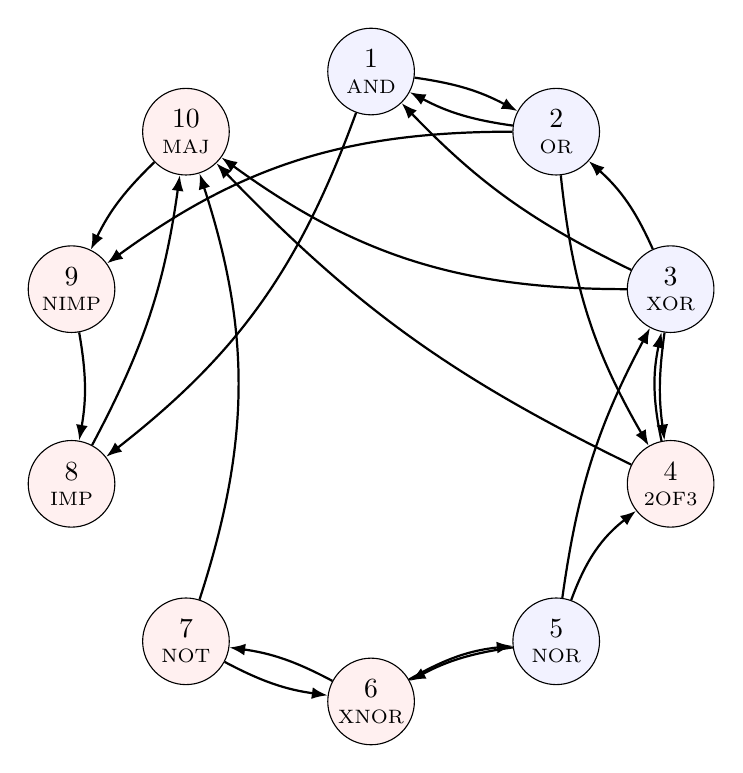
\begin{tikzpicture}[
  gate/.style={circle, draw, minimum size=11mm, align=center, inner sep=1pt, fill=blue!5},
  focus/.style={circle, draw, minimum size=11mm, align=center, inner sep=1pt, fill=red!6},
  >={Latex[length=2mm]}
]
\node[gate]  (n1)  at (90:4.0)   {1\\[-1mm]\scriptsize AND};
\node[gate]  (n2)  at (54:4.0)   {2\\[-1mm]\scriptsize OR};
\node[gate]  (n3)  at (18:4.0)   {3\\[-1mm]\scriptsize XOR};
\node[focus] (n4)  at (-18:4.0)  {4\\[-1mm]\scriptsize 2OF3};
\node[gate]  (n5)  at (-54:4.0)  {5\\[-1mm]\scriptsize NOR};
\node[focus] (n6)  at (-90:4.0)  {6\\[-1mm]\scriptsize XNOR};
\node[focus] (n7)  at (-126:4.0) {7\\[-1mm]\scriptsize NOT};
\node[focus] (n8)  at (-162:4.0) {8\\[-1mm]\scriptsize IMP};
\node[focus] (n9)  at (162:4.0)  {9\\[-1mm]\scriptsize NIMP};
\node[focus] (n10) at (126:4.0)  {10\\[-1mm]\scriptsize MAJ};
\draw[->, thick] (n2) to[bend left=10] (n1);
\draw[->, thick] (n3) to[bend left=10] (n1);
\draw[->, thick] (n1) to[bend left=10] (n2);
\draw[->, thick] (n3) to[bend right=12] (n2);
\draw[->, thick] (n4) to[bend left=12] (n3);
\draw[->, thick] (n5) to[bend left=10] (n3);
\draw[->, thick] (n2) to[bend right=12] (n4);
\draw[->, thick] (n3) to[bend right=8] (n4);
\draw[->, thick] (n5) to[bend left=16] (n4);
\draw[->, thick] (n6) to[bend left=12] (n5);
\draw[->, thick] (n5) to[bend right=10] (n6);
\draw[->, thick] (n7) to[bend right=10] (n6);
\draw[->, thick] (n6) to[bend right=10] (n7);
\draw[->, thick] (n1) to[bend left=16] (n8);
\draw[->, thick] (n9) to[bend left=10] (n8);
\draw[->, thick] (n2) to[bend right=18] (n9);
\draw[->, thick] (n10) to[bend right=10] (n9);
\draw[->, thick] (n3) to[bend left=18] (n10);
\draw[->, thick] (n4) to[bend left=10] (n10);
\draw[->, thick] (n7) to[bend right=18] (n10);
\draw[->, thick] (n8) to[bend right=10] (n10);
\end{tikzpicture}
\caption{Ten-node mixed-gate benchmark network.  Blue nodes use monotone
or parity gates; red nodes use threshold, negation, implication, or
majority gates.}
\label{fig:10node-network}
\end{figure}

The connected-input sets are extracted from the connectivity matrix, and
each node's analytic one-set is computed via \texttt{indexSetAnalytic} and
verified against the exhaustive baseline on all $2^{10}=1024$ rows:

\begin{lstlisting}[style=MathematicaStyle,caption={Per-node verification against exhaustive baseline.}]
ics10 = Table[Sort@Flatten@Position[cm10[[k]], 1],
              {k, 1, 10}];
oneSets10 = Table[
  Sort@indexSetAnalytic[10, ics10[[k]],
    dyn10[[k]], Lookup[params10, k, <||>]],
  {k, 1, 10}];
baselineOneSets10 = Table[
  Flatten@Position[outputs10[[All, k]], 1],
  {k, 1, 10}];

And @@ Table[Sort[oneSets10[[k]]] ===
             Sort[baselineOneSets10[[k]]], {k, 1, 10}]
\end{lstlisting}
\begin{lstlisting}[style=MathematicaOutput]
(* Connected input sets:                                *)
(*   Node 1 (AND): {2,3}   Node 6 (XNOR): {5,7}       *)
(*   Node 2 (OR):  {1,3}   Node 7 (NOT):  {6}          *)
(*   Node 3 (XOR): {4,5}   Node 8 (IMP):  {1,9}        *)
(*   Node 4 (KOFN):{2,3,5} Node 9 (NIMP): {2,10}       *)
(*   Node 5 (NOR): {6}     Node 10(MAJ):  {3,4,7,8}    *)
(* Per-node verification:                               *)
(*   {True,True,True,True,True,True,True,True,True,True}*)
(* Out: True                                            *)
\end{lstlisting}

All ten gates---AND, OR, XOR, KOFN, NOR, XNOR, NOT, IMPLIES, NIMPLIES,
and MAJORITY---pass: the analytic one-sets coincide exactly with the
exhaustive output columns produced by \texttt{ApplyGate}.

We then define six mixed queries---four full-output patterns and two
subsystem projections---and compute their compressed representations
via \texttt{mixedQueryRepresentation}, which intersects local one-sets
and extracts the base set and offset family:

\begin{lstlisting}[style=MathematicaStyle,caption={Mixed-query evaluation and corroboration.}]
queryIndices[nodes_, pattern_] := Sort@Fold[
  Intersection, Range[2^10],
  MapThread[
    If[#2 == 1, oneSets10[[#1]],
       Complement[Range[2^10], oneSets10[[#1]]]] &,
    {nodes, pattern}]];

mixedQueryRepresentation[nodes_, pattern_] := Module[
  {analytic, unionCoords, sumandos, baseIndices},
  analytic = queryIndices[nodes, pattern];
  unionCoords = Sort@DeleteDuplicates@
    Flatten[ics10[[nodes]]];
  sumandos = allOffsets[10, unionCoords];
  baseIndices = Select[analytic,
    Function[idx, AllTrue[
      Complement[Range[10], unionCoords],
      inputs10[[idx, #]] == 0 &]]];
  <|"DecimalRepertoire" -> baseIndices,
    "Sumandos" -> sumandos|>];

resF1 = mixedQueryRepresentation[Range[10],
           {1,1,1,1,1,1,1,1,1,1}];
gpF1  = givePlaces[resF1["DecimalRepertoire"],
                   resF1["Sumandos"]];
Sort[gpF1] === Sort[queryIndices[Range[10],
                {1,1,1,1,1,1,1,1,1,1}]]
\end{lstlisting}
\begin{lstlisting}[style=MathematicaOutput]
(* F1 DecimalRepertoire: {143,215,399,400,471,472}    *)
(* F1 Sumandos:          {0}                          *)
(* F1 Unfolded:          {143,215,399,400,471,472}    *)
(* Out: True  [verified for all six cases F1-F4,S1,S2]*)
\end{lstlisting}

Tables~\ref{tab:full-cases} and~\ref{tab:subsystem-cases} show the
results for all six cases.  Every value shown is the actual output of
the code above.

\begin{table}[h]
\centering
\small
\setlength{\tabcolsep}{3pt}
\begin{adjustbox}{max width=\textwidth,center}
\begin{tabular}{@{}lcccc@{}}
\toprule
Case & Output pattern & DecimalRepertoire & Sumandos & Rows \\
\midrule
F1 & \texttt{1111111111} & $\{143,215,399,400,471,472\}$ & $\{0\}$ & 6 \\
F2 & \texttt{1111111110} & $\{15,87,271,272,343,344\}$ & $\{0\}$ & 6 \\
F3 & \texttt{1111111101} & $\{655,727,911,912,983,984\}$ & $\{0\}$ & 6 \\
F4 & \texttt{1111101111} & $\{79,207,335,336,463,464\}$ & $\{0\}$ & 6 \\
\bottomrule
\end{tabular}
\end{adjustbox}
\caption{Compressed representation for the four full-output queries.
Each case yields exactly 6 satisfying rows out of 1024.  Because the
full-output queries saturate all 10 coordinates ($C_q = [10]$, no free
coordinates), the offset family is $\{0\}$ and the DecimalRepertoire
\emph{is} the complete one-set.}
\label{tab:full-cases}
\end{table}

\begin{table}[h]
\centering
\small
\setlength{\tabcolsep}{3pt}
\begin{adjustbox}{max width=\textwidth,center}
\begin{tabular}{@{}lcccc@{}}
\toprule
Case & Queried nodes / pattern & DecimalRepertoire & Sumandos & Rows \\
\midrule
S1 & $\{4,6,7,10\}$ / \texttt{0111} & $\{141,217\}$ &
  $\{0,1,256,257,512,513,768,769\}$ & 16 \\
S2 & $\{4,6,7,8,9,10\}$ / \texttt{011101} &
  $\{141,217,397,398,473,474,$ &
  $\{0\}$ & 12 \\
   & & $653,729,909,910,985,986\}$ & & \\
\bottomrule
\end{tabular}
\end{adjustbox}
\caption{Compressed representation for the subsystem queries.
$S1$ has free coordinates $\{1,9,10\}$, so the 2-element base set
unfolds via 8 offsets to 16 rows.
$S2$ saturates all 10 coordinates, collapsing to a 12-element base set
with trivial offsets.
All indices verified exactly against the exhaustive baseline.}
\label{tab:subsystem-cases}
\end{table}


\subsection{Overlap analysis}\label{sec:overlap}

The six query cases reveal the role of overlapping input supports.
When several queried nodes share input coordinates, the effective
search space shrinks from the sum of their local arities to the size
of the coordinate union.

Define:
\begin{itemize}
\item $d_q = \sum_{i\in Q}|N_i|$: the sum of queried gate arities
  (the ``raw'' local-assignment space has size $2^{d_q}$).
\item $c_q = |C_q|$: the size of the union of their connected-input
  coordinates.
\item $\mu_q = d_q - c_q$: the \emph{overlap multiplicity}, counting
  repeated coordinate uses.
\item $R_q = 2^{\mu_q}$: the exact reduction factor.
\end{itemize}

\begin{table}[h]
\centering
\small
\begin{tabular}{@{}lcccccl@{}}
\toprule
Case & Queried nodes & $d_q$ & $c_q$ & $\mu_q$ & $R_q$ & $C_q$ \\
\midrule
F1--F4 & $\{1,\ldots,10\}$ & 21 & 10 & 11 & $2048$ & $\{1,\ldots,10\}$ \\
S1 & $\{4,6,7,10\}$ & 10 & 7 & 3 & $8$ & $\{2,3,4,5,6,7,8\}$ \\
S2 & $\{4,6,7,8,9,10\}$ & 14 & 10 & 4 & $16$ & $\{1,\ldots,10\}$ \\
\bottomrule
\end{tabular}
\caption{Overlap statistics for the mixed queries.  The full-output queries
have $d_q=21$ (the sum of all local arities) but $c_q=10$ (only 10 distinct
coordinates exist), giving an overlap multiplicity of $\mu_q=11$ and an
exact reduction factor of $R_q=2^{11}=2048$.}
\label{tab:overlap-stats}
\end{table}

The most transparent case is $S1$.  The four queried gates contribute
$3+2+1+4=10$ local inputs, but their coordinate union is only
$C_{S1}=\{2,3,4,5,6,7,8\}$ (seven coordinates).  The three free
coordinates $F_{S1}=\{1,9,10\}$ generate the offset family
\[
\Omega(F_{S1}) = \{0,1,256,257,512,513,768,769\},
\]
and the zero-free base set is $L_{S1}^{(0)}=\{141,217\}$.  Deconvolution
then gives
\[
\mathcal{J}_{S1} = \operatorname{Dec}(\{141,217\},\,\Omega(\{1,9,10\})),
\]
which unfolds to the 16 corroborated rows.  This is the exact multi-gate
analogue of the single-gate AND deconvolution: overlap first shrinks the
determining coordinate set from 10 to 7, and only then do the remaining
free coordinates generate the full family of offsets.


\subsection{What the compression reveals}\label{sec:compression-reveals}

Three structural observations emerge from the overlap analysis.

First, the full-output queries saturate all ten coordinates
($C_q = \{1,\ldots,10\}$), leaving no free coordinates.  The offset
family therefore collapses to the singleton $\{0\}$, and the
DecimalRepertoire \emph{is} the complete answer set.  This is the
limiting case of causal compression: the query is so tightly constrained
that the base set alone suffices, and the analytic path reduces the raw
$2^{21}$-element local-assignment space to a direct enumeration of the
few satisfying rows.  The four cases F1--F4 each yield exactly six rows
out of 1024, and their DecimalRepertoire sets differ precisely in those
six positions---the topological skeleton is shared, but the gate-specific
selection rules pick out different decimal anchors.

Second, even though the full-output queries have trivial offsets, they
still benefit from overlap: the raw local-assignment space drops from
$2^{21}$ to $2^{10}$, an exact reduction factor of $2^{11}=2048$, before
any row materialisation is considered.  The query does not pay once per
gate for a shared coordinate; it pays once for the coordinate itself.

Third, what appears in the full repertoire as dispersed behaviour---six
rows scattered across 1024---is explained analytically as overlap-aware
reuse of shared coordinates.  The compressed representation makes the
generative structure visible, whereas the exhaustive table presents only
the effect.  The subsystem query $S1$ illustrates the complementary case:
with three free coordinates, its two-element base set unfolds via eight
offsets to 16 rows, showing how the offset family encodes the degrees of
freedom that the query leaves unconstrained.


%%% ===========================================================================
\section{Scalability and Causal Compression}\label{sec:scalability}
%%% ===========================================================================

\subsection{Resource-envelope benchmarks}\label{sec:benchmarks}

The scalability of the analytic method depends on the support-union size
$|C_q|$, not on the ambient network size $n$.  To confirm this, a
deterministic benchmark was executed across ring-local heterogeneous
Boolean networks at $n\in\{30,60,80,200\}$, with five independently
seeded replicates per size.  The gate catalogue covered all eleven
non-canalising families.  Three query tiers were measured:

\begin{itemize}
\item \textbf{T1} ($|Q|=1$): a single queried node.
\item \textbf{T2} ($|Q|=4$): a four-node query.
\item \textbf{T3} ($|Q|=8$): an eight-node query (the primary stress case).
\end{itemize}

\begin{table}[h]
\centering
\small
\begin{tabular}{rrrrrrr}
\toprule
$n$ & Query & $|C_q|$ & $n{-}|C_q|$ & $\mu_q$ & Time (s) & Peak memory \\
\midrule
 30 & T1 &  3 &  27 &  0 & $6.7\times10^{-5}$ &  4.3\,KB \\
 30 & T2 &  7 &  23 &  4 & $2.4\times10^{-4}$ & 12.2\,KB \\
 30 & T3 & 10 &  20 & 13 & $4.7\times10^{-4}$ & 14.4\,KB \\
\midrule
 60 & T1 &  3 &  57 &  0 & $6.4\times10^{-5}$ &  4.1\,KB \\
 60 & T2 &  5 &  55 &  5 & $2.0\times10^{-4}$ &  8.7\,KB \\
 60 & T3 & 10 &  50 & 10 & $9.7\times10^{-4}$ & 33.4\,KB \\
\midrule
 80 & T1 &  4 &  76 &  0 & $1.1\times10^{-4}$ &  7.6\,KB \\
 80 & T2 &  6 &  74 &  4 & $1.9\times10^{-4}$ &  7.3\,KB \\
 80 & T3 & 10 &  70 & 10 & $5.5\times10^{-4}$ & 18.2\,KB \\
\midrule
200 & T1 &  3 & 197 &  0 & $6.2\times10^{-5}$ &  4.1\,KB \\
200 & T2 &  6 & 194 &  3 & $2.2\times10^{-4}$ &  8.8\,KB \\
200 & T3 & 10 & 190 & 10 & $1.1\times10^{-3}$ & 34.9\,KB \\
\bottomrule
\end{tabular}
\caption{Executed exact causal evaluation measurements (median over five
replicates per size).  All measurements remain in the sub-millisecond to
low-millisecond range across the full range $n=30$ to $n=200$, confirming
that the cost is governed by $|C_q|$ rather than by $n$.}
\label{tab:resource-envelope}
\end{table}

The central observation is that the median support-union size $|C_q|$ for
the T3 tier remains approximately $10$ across all four ambient sizes.  As
$n$ grows from 30 to 200, the free-coordinate count grows from 20 to
190---the region the exact method avoids enumerating---while wall time
fluctuates only within the sub-millisecond to low-millisecond range.

Table~\ref{tab:synthesis} contrasts the exact method against the naive
exhaustive lower bounds.

\begin{table}[h]
\centering
\small
\begin{tabular}{rrrrr}
\toprule
$n$ & Exact time (s) & Exact memory
    & Naive storage LB & Naive time LB \\
\midrule
 30 & $4.7\times10^{-4}$ & 14.4\,KB
    & 3.75\,GB                  & ${\approx}1.07$\,s \\
 60 & $9.7\times10^{-4}$ & 33.4\,KB
    & 7.50\,EB                  & ${\approx}36.5$\,y \\
 80 & $5.5\times10^{-4}$ & 18.2\,KB
    & 10.0\,YB                  & ${\approx}3.83\times10^{7}$\,y \\
200 & $1.1\times10^{-3}$ & 34.9\,KB
    & ${\approx}4.02\times10^{61}$\,B & ${\approx}5.09\times10^{43}$\,y \\
\bottomrule
\end{tabular}
\caption{Synthesis comparison for the T3 tier (median over five
replicates).  Naive storage lower bound is $n\,2^n/8$ bytes; naive time
lower bound extrapolates at $10^9$ rows per second.  At $n=60$ naive
materialisation exceeds the exabyte threshold; at $n=200$ it exceeds any
physically realised medium by many orders of magnitude.}
\label{tab:synthesis}
\end{table}


\subsection{Description length and causal compression}\label{sec:description-length}

A conceptually distinct comparison concerns the description length of the
mechanism versus the complexity of the materialised output.  The underlying
principle, explored computationally in~\cite{hernandez2019}, is that
algorithmically simple objects---those generated by short programmes---are
\emph{sensitive} to perturbation: modifying a single instruction in the
generating programme produces non-linear changes in the output, because the
programme's parts are causally interdependent.  By contrast, algorithmically
random objects are \emph{insensitive}: their shortest description is the
object itself, and random perturbations change only a small fraction of
the data.  The ratio between the length of the generating programme and the
length of its output is therefore a quantitative signature of causal
structure.

\paragraph{The encoding.}
Because a description length is meaningless until the descriptive language is
fixed, we state ours explicitly.  Each node $i$ of a network of size $n$,
carrying gate $g_i$ with in-degree $d_i$, is encoded by three fields:
\[
\underbrace{\log_2 K}_{\text{which gate}}
\;+\;
\underbrace{\log_2 (n+1)}_{\text{in-degree } d_i}
\;+\;
\underbrace{\log_2\!\binom{n}{d_i}}_{\text{which inputs}}
\;+\;
\underbrace{\pi(g_i,d_i,n)}_{\text{parameters}},
\qquad K=12,
\]
and $D_{\mathrm{formula}}=\sum_{i=1}^{n}$ of these costs.  The parameter field
$\pi$ charges what each family actually requires: $\log_2(d_i+1)+1$ for KOFN
(the threshold $k\in\{0,\ldots,d_i\}$), $\log_2 n+2$ for CANALISING (canalising
index, canalising value, canalised output), $\log_2\max(1,d_i(d_i-1))$ for
IMPLIES and NIMPLIES (an \emph{ordered} pair among the inputs),
$\log_2\max(1,d_i)$ for NOT, and a uniform one-bit polarity slot otherwise.
Costs are idealised code lengths and are not rounded to whole bits.

The in-degree field is not decorative: without $d_i$ a decoder can neither
determine how many bits to read for the input set nor interpret them as an index
into the $d_i$-subsets of $\{1,\ldots,n\}$, so a code lacking it is not uniquely
decodable and is therefore not a description length at all.  The cost of
specifying $n$ itself is not charged, being constant across the networks
compared here.

One property of this encoding must be stated plainly: it is a declared
\emph{choice}, not a canonical object.  The
invariance theorem guarantees only that a change of descriptive framework costs
an additive constant, and in applications that constant can be arbitrarily
large~\cite{zenildecomposition}.  What the present setting secures is narrower
and still worth stating: because the mechanism is given and the encoding is
published, the constant is fixed and known rather than unknown and unbounded, so
figures computed this way are exactly comparable across networks.
$D_{\mathrm{formula}}$ is accordingly an upper bound on the shortest description
in one declared language---never an estimate of $K$.

\paragraph{Measured values.}
For the 10-node benchmark:

\begin{center}
\small
\begin{tabular}{@{}p{0.34\linewidth}p{0.15\linewidth}p{0.38\linewidth}@{}}
\toprule
\textbf{Measure} & \textbf{Value} & \textbf{Interpretation} \\
\midrule
Formula components $C_{\mathrm{formula}}$ & $23$
  & symbolic pieces in the analytic description \\
Programme length $D_{\mathrm{formula}}$ & $135.66$ bits
  & the mechanism, under the encoding above \\
BDM of the output & $580.01$ bits
  & algorithmic estimate of the behaviour \\
ZIP-compressed output & $10\,016$ bits
  & lossless compression of the output table \\
Shannon content $H_{\mathrm{total}}$ & $10\,229.61$ bits
  & repertoire-scale i.i.d.\ coding \\
$D_{\mathrm{formula}}/\mathrm{BDM}$ & $0.234$
  & estimator within a small factor of the truth \\
$D_{\mathrm{formula}}/\mathrm{ZIP}$ & $1.35\times10^{-2}$
  & mechanism two orders of magnitude smaller \\
$D_{\mathrm{formula}}/H_{\mathrm{total}}$ & $1.33\times10^{-2}$
  & mechanism is far shorter than full coding \\
\bottomrule
\end{tabular}
\end{center}

The exact formulae are not merely another way to print the same table:
they constitute a dramatically shorter generative description.
$D_{\mathrm{formula}}$ measures the cost of specifying the mechanism;
$\mathrm{ZIP}$ and $H_{\mathrm{total}}$ measure the cost of describing what that
mechanism produces.  The load-bearing comparison is with $\mathrm{ZIP}$, since a
general-purpose compressor is a genuine adversary: it is free to exploit any
regularity it can find in the realised outputs, and it still requires two orders
of magnitude more bits than the generative law.

$H_{\mathrm{total}}$ deserves a caveat rather than emphasis.  At $10\,229.61$
bits it is $99.9$ per cent of the raw $10\,240$-bit table, because the output
bits are close to balanced and an entropy code therefore saves almost nothing.
Far from weakening the result, this is the sharpest way to state it: the
behaviour of this network is \emph{statistically near-featureless} and
nevertheless generated by a description of a hundred bits.  Statistical
featurelessness and extreme algorithmic compressibility coexist here, which is
precisely the regime in which distributional summaries are least informative and
generative descriptions most so.

\paragraph{Calibrating an algorithmic estimator against known ground truth.}
Comparing a generative law only against statistical baselines would be a weak
test, since it selects opponents that are constitutionally unable to see
generative structure.  The stronger comparison is with a method designed to
estimate algorithmic content without knowing the mechanism.  We therefore
compute the Block Decomposition Method (BDM)~\cite{zenildecomposition} over the
same $2^{10}\times 10$ output repertoire.  Because the generating programme and
its exact length are both known here, this is a rare setting: the estimator can
be assessed against ground truth rather than against another estimate.

BDM returns $580.01$ bits, against $10\,016$ for ZIP and $10\,229.61$ for
$H_{\mathrm{total}}$.  The algorithmic estimator is thus roughly seventeen times
more efficient than lossless compression on an object where compression is
nearly powerless, which is a substantial vindication of the algorithmic
approach over the statistical one.  Two controls confirm that BDM is responding
to the generative structure and not to the marginals: a row permutation, which
preserves every row of the table and destroys only the ordering geometry,
raises BDM to $14\,714$ bits; and a density-matched random matrix gives
$15\,545$ bits.  The separations are $25.4$-fold and $26.8$-fold respectively,
and they are robust to the choice of partition strategy.\footnote{All values use
a recursive partition covering every column.  The default block partition in
common implementations discards leftover columns---at $n=10$ it silently
measures eight of the ten---and we report the recursive figure throughout.  BDM
is also known to converge toward Shannon entropy once block sizes outrun the
available CTM tables, so these values should be read as scale-dependent
estimates.}

The residual gap is the quantity of interest.  At $580.01$ bits against a true
programme length of $135.66$, BDM sits within a factor of $4.3$ of the exact
description.  That factor is a measure of the price of not knowing the
generator: it is what an estimator must pay when the mechanism has to be
recovered from the output rather than read off from the specification.  It is
small, which speaks well of the estimator, and it is not zero, which is what one
should expect of any method that must infer rather than compute.  The
significance of the present setting is that this factor can be measured at all.

Where the remaining gap comes from is also visible.  Block decomposition
combines local estimates with a global account of repetition, so structure
that spans blocks must be paid for once per occurrence; recent work extends
the method with reusable program code and conditional descriptions precisely
to charge shared structure only once~\cite{sakabe2026reusable}.  The
representation studied here is the limiting case of that idea.  The base set
$L$ is the code, written once; the offset family $\Omega$ is the schedule of
its reuse, and because $\Omega$ factorises as a sumset of the free weights the
schedule is itself given in closed form rather than discovered.  An estimator
must infer both the code and the schedule from the output; here the mechanism
supplies them.  That is the whole of the difference between $135.66$ and
$580.01$ bits, and it is why the comparison is a calibration rather than a
competition.  Appendix~\ref{app:gate-bdm} applies the same estimator at the
level of a single gate definition, where it serves as a check on the
representation rather than on the method.

\medskip
This is causal compression in a precise, non-rhetorical sense: the 23 formula
components form a short programme whose output spans 1024 rows and 206
distinct output states.

A single experiment fixes what the two sides of that statement do and do not
measure, and forestalls the most natural misreading.  Rewire node 10 to a
different input set of the same cardinality.  The behaviour changes
substantially: 440 of the 1024 output rows differ, and the number of distinct
output states falls from 206 to 172.  The description length does not change
at all---$D_{\mathrm{formula}}$ is bit-identical, because it is a function of
$n$, the in-degrees and the gate types alone and never reads an output bit.
Both facts are consequences of the same design.  $D_{\mathrm{formula}}$ is the
correct quantity for the programme side of a programme-versus-output
comparison, and it is not a complexity measure of behaviour: it cannot rank
networks by the richness of what they do, and no claim of that form is made
here.  The behavioural side of the comparison is carried by BDM, ZIP and
$H_{\mathrm{total}}$, which respond to the realised output and not to the
specification.


%% ARTEFACT-BEGIN comp_validation_summary (producers: TSK-ALGO-004-ClosedFormSetAudit.m Metrics.json + complexity_analysis.py)
\subsection{Validation summary}\label{sec:validation}

Exact reconstruction has been verified at $n=10$ and $n=13$ by exhaustive
comparison against the baseline repertoire, and beyond the exhaustive-baseline
range at $n\in\{16,20\}$ by a stratified closed-form-set audit across all twelve
gate families (seeds 301 and 302): each node's packaged closed-form one-set is
materialised and compared entry-by-entry against the full gate truth table over
all $2^{d}$ connected-input patterns, and the composed analytic prediction is
checked row-wise against direct evaluation on 1020 Hamming-stratified rows per
seed, with zero elementwise mismatches in all cases. A dispatch-consistency
audit additionally covers $n\in\{20,50\}$ (1020 stratified rows, seeds 201 and
202); it validates large-scale evaluation plumbing and carries no theorem weight.
%% ARTEFACT-END comp_validation_summary

\begin{table}[h]
\centering
\small
\begin{tabular}{@{}p{0.28\linewidth}p{0.20\linewidth}p{0.28\linewidth}p{0.10\linewidth}@{}}
\toprule
\textbf{Claim} & \textbf{Validation layer} & \textbf{Evidence} & \textbf{Scale} \\
\midrule
Gate one-set exactness &
Gate algebra; property tests &
Per-gate corroboration &
$|N_i|\leq 6$ \\[3pt]
Ordering invariance &
Six-node check &
Involution transport &
$n=6$ \\[3pt]
Network exactness &
Dispatch consistency &
Zero discrepancy; accuracy $1.0$ &
$n\leq 13$ \\[3pt]
Cost governed by $|C_q|$ &
Resource-envelope benchmark &
Tables~\ref{tab:resource-envelope}--\ref{tab:synthesis} &
$n\leq 200$ \\[3pt]
Sampling reduces validation cost &
Stratified sampled audit &
Accuracy $1.0$; seeds 301, 302 &
$n\in\{20,50\}$ \\
\bottomrule
\end{tabular}
\caption{Mapping from claims to validation evidence.}
\label{tab:validation-map}
\end{table}


%%% ===========================================================================
\section{Dynamical Landscape}\label{sec:dynamics}
%%% ===========================================================================

The previous sections answered an exact inverse question: which input rows
produce selected mixed output events.  We now add the complementary
forward-dynamical question on the same 10-node network: which output
patterns are themselves one-step realisable, and which belong to the
recurrent part of the state-transition graph?

%% ARTEFACT-BEGIN w05_comp_attractor_stats (producer: papers/method/manuscript_computational/generate_paper_outputs.wl -> dynamical_landscape.json)
Let $F:\bits^{10}\to\bits^{10}$ be the synchronous update map.  Exhaustive
enumeration of all $2^{10}=1024$ states gives
\[
|\mathrm{Im}(F)| = 206,
\qquad
|\mathcal{U}_{10}\setminus\mathrm{Im}(F)| = 818,
\qquad
\frac{|\mathrm{Im}(F)|}{|\mathcal{U}_{10}|} \approx 0.201.
\]
Only about $20.1\%$ of all 10-bit patterns are admissible as one-step
outputs.  The local logical constraints and the overlap structure restrict
the forward image to a small structured subset of the full configuration
space.

The recurrent dynamics collapse further.  Table~\ref{tab:attractors} shows
that the entire functional graph has only four attractors: one fixed point,
two 2-cycles, and one 6-cycle.

\begin{table}[h]
\centering
\small
\begin{tabular}{cccc}
\toprule
Attractor & Period & Basin size & Recurrent states \\
\midrule
$A_1$ & 1 & 488 & $\{$\texttt{0000010100}$\}$ \\
$A_2$ & 2 & 320 & $\{$\texttt{1101010110}, \texttt{0110010110}$\}$ \\
$A_3$ & 6 & 204 & $\{$\texttt{1111010101}, \texttt{1111010001}, \texttt{1111010000},\\
      &   &     & \phantom{$\{$}\texttt{1111010010}, \texttt{1111010110}, \texttt{1111010111}$\}$ \\
$A_4$ & 2 & 12  & $\{$\texttt{1111010100}, \texttt{1111010011}$\}$ \\
\bottomrule
\end{tabular}
%% ARTEFACT-END w05_comp_attractor_stats
\caption{Exact recurrent structure of the 10-node benchmark.  Basin sizes
sum to 1024; the three largest basins cover $98.8\%$ of the state space.}
\label{tab:attractors}
\end{table}

The connection between the exact causal queries and the dynamical landscape
is immediate.  The four full-output patterns $F1$--$F4$ are all one-step
reachable states, but none is itself an attractor state.  Cases $F1$--$F3$
converge to the 2-cycle $A_2$ within three steps; $F4$ converges to the
fixed point $A_1$ within six steps.  The subsystem query $S1$ induces five
distinct image states spread across all four basins; adding the extra $S2$
constraints narrows this to three image states in three basins, removing
the branch to $A_4$.  Stronger exact causal constraints reduce not only
combinatorial freedom but also dynamical dispersion.

The causal descriptions (backward query) and the dynamical landscape
(forward iteration) are complementary views of the same network.  The
backward query identifies the generative structure---which input conditions
produce a given event.  The forward dynamics reveal the eventual fate of
those events under iterated application of the same causal rules.  Neither
view alone exhausts the network's behaviour; together they provide both
mechanism and consequence.

In the language of AID, the backward query is a perturbation test: the
system is interrogated about its own computational capabilities, and the
compressed representation is its answer.  The forward dynamics show that
this answer has further consequences: the six rows satisfying $F1$ do not
scatter randomly through the state-transition graph but converge to a
specific attractor within three steps.  The causal rules that determine
\emph{which} input conditions produce a given output also determine
\emph{where} that output leads under iteration---the mechanism governs both
the generative and the consequential structure of the network.


%%% ===========================================================================
\section{Discussion}\label{sec:discussion}
%%% ===========================================================================

The central contribution of this paper is the formalisation and
computational validation of a causal compression methodology for Boolean
networks.  The methodology rests on the observation that deterministic
local rules imprint self-similar patterns across the exhaustive
repertoire, and that these patterns admit exact short descriptions.
We discuss the principal results and their connections to the broader
programme of algorithmic causality.

\textbf{General formulae for all gate families.}  The self-similar
patterns first observed empirically for AND, OR, and XOR
gates~\cite{hernandez2019} turn out to have a uniform algebraic
structure that holds across all twelve canonical families.  Each gate
type determines a characteristic selection rule over the connected-input
assignments---band intersections for monotone gates, parity classes for
XOR/XNOR, Hamming-weight layers for threshold gates, asymmetric pairs
for implication, hierarchical collapse for canalising gates---while the
offset family generated by disconnected coordinates is identical for all
gates sharing the same topology.  This separation is not a coincidence;
it reflects the factorisation of the network's causal structure into a
gate-semantic component (the base set) and a topological component (the
offset family).  Together they constitute a short generative programme
for the full one-set of any gate.

\textbf{Overlap compression.}  When multiple nodes are queried
simultaneously, shared input coordinates reduce the effective search space
by an exact factor of $2^{\mu_q}$.  For the 10-node benchmark, this factor
reaches $2048$ for the full-output queries.  The compressed representation
makes this reduction explicit: the base set encodes the constrained
coordinates, the offset family encodes the free coordinates, and
deconvolution recovers the full answer.
The full-output queries illustrate the limiting case: all coordinates are
constrained, the offset family collapses to $\{0\}$, and the
DecimalRepertoire alone constitutes the complete answer.

\textbf{Scalability.}  The analytic evaluation cost is governed by
$|C_q|$, not by $n$.  Under bounded in-degree and bounded query scope,
median analytic evaluation stays at or below roughly a millisecond at
$n=200$, a regime where naive exhaustive materialisation is physically
impossible; the salient fact is not the absolute figure, which is
hardware-dependent, but that it is indistinguishable from the figure at
$n=30$.  In the language of
Section~\ref{sec:gate-families} this is a statement about schema order: what
must be evaluated is the number of fixed positions, not the size of the space
in which they sit.

\textbf{The method as the exactly solvable limit of AID.}  The
methodology realises the AID
principle~\cite{zenilcalculus,zenildeconv,zenilaidbook} that short
generative descriptions of complex behaviour can be identified by
exploiting the causal structure of the generating mechanism---but it does so
in the restricted regime where the mechanism is given rather than inferred.
The compressed representation is the ``short programme''; the full
repertoire is the ``complex output''; and the two-orders-of-magnitude gap
between $D_{\mathrm{formula}}$ and the cost of describing the behaviour is a
quantitative measure of causal compression.

Because the mechanism is known here, no estimator is needed and none is
proposed.  The methodological contribution runs in the other direction: the
networks studied here are objects whose exact generating programme and exact
description length are both available, which makes them a calibration class
for methods that must operate without that knowledge.
Section~\ref{sec:description-length} uses them so, and the outcome is
informative in a way that a purely internal comparison could not be---the
algorithmic estimator recovers the structure that statistical measures miss
entirely, and lands within a small constant factor of the true programme
length.

The connection to perturbation analysis is direct: a system whose causal
description is short is one whose output changes non-linearly under
perturbation of the generating programme~\cite{hernandez2019}, as the
rewiring experiment of Section~\ref{sec:description-length} shows
concretely.  This sensitivity is the hallmark of an algorithmically simple,
causally integrated system---precisely the regime in which the methodology is
most powerful.  The density-matched random control of the same section is the
opposite pole: an object with no short causal description, on which the method
would offer no compression advantage and on which, as measured, the
algorithmic estimator itself returns a value close to the raw size.

\textbf{Connection to Wolfram.}  The Principle of Computational
Equivalence~\cite{wolfram2002new} holds that simple rules generate rich
behaviour.  The present method makes this quantitative: the 10-node
network is specified by 23 formula components, yet its full behaviour spans
1024 rows with 206 distinct output states, 4 attractors, and structured
basin geometry.  The causal description is short; the generated behaviour
is complex.

\textbf{Limitations.}  The computational advantage depends on bounded
support size: when $|C_q|$ approaches $n$, the analytic path converges to
the cost of exhaustive materialisation.  The method is therefore most
powerful for networks with bounded in-degree and localised query scope.
The present formalism treats synchronous one-step update; asynchronous or
stochastic schedules are a direction for future work.

Three qualifications attach to the description-length results specifically.
First, $D_{\mathrm{formula}}$ is a length under one declared encoding, an
upper bound on the shortest description in that language and not an estimate
of $K$; a different but equally reasonable encoding would shift it by a
constant.  Second, the calibration of
Section~\ref{sec:description-length} is performed on a single network at a
single scale, and the factor of $4.3$ should be read as one measurement
rather than a general constant; establishing how that factor behaves across
network families, sizes and in-degree regimes is the natural next study, and
the present method supplies the ground truth such a study would require.
Third, the estimator itself is scale-dependent, converging toward Shannon
entropy once block sizes outrun the available base tables, so the comparison
is meaningful in the regime reported and should not be extrapolated beyond it
without re-measurement.


%%% ===========================================================================
\section{Conclusion}\label{sec:conclusion}
%%% ===========================================================================

We have presented a causal compression methodology for Boolean networks
that derives exact short descriptions of network behaviour from the
interaction between gate semantics and network topology, validated
computationally across all twelve canonical gate families, overlap-aware
multi-node queries, and networks of up to $n=200$ nodes.

The method rests on a uniform decomposition: every gate family determines a
base set over its connected inputs, and every topology generates an offset
family from its disconnected coordinates.  Deconvolution of this pair
recovers the exact one-set without row-wise gate evaluation.  When multiple
nodes are queried, overlapping input supports compress the effective search
space by an exact factor of $2^{\mu_q}$.

The computational characterisation confirms that analytic evaluation remains
of the order of a millisecond at $n=200$ under bounded in-degree, and
does not grow with $n$, that the causal
description ($D_{\mathrm{formula}}=135.66$ bits) is two orders of magnitude
shorter than any statistical encoding of the realised outputs
($\mathrm{ZIP}=10\,016$ bits, $H_{\mathrm{total}}=10\,229.61$ bits) while a
block-decomposition estimator, given no access to the mechanism, recovers the
structure to within a factor of $4.3$, and that all results are verified
exactly against exhaustive baselines at tractable sizes.

The causal descriptions (backward query) and the dynamical landscape
(forward iteration) provide complementary views of the same network.
Together, they demonstrate that complex Boolean-network behaviour can be
represented and reconstructed by short exact causal formulae.  The
compressed representation is not merely a computational shortcut; it
identifies the generative structure of the mechanism---the short programme
whose execution produces the observed behaviour.  This is causal
compression in the precise sense of the Algorithmic Information Dynamics
programme~\cite{zenilcalculus}: the network admits a description that is
dramatically shorter than its output, and this brevity is a direct
consequence of the deterministic causal rules that generate it.

The method provides a general tool for any domain in which Boolean
networks model discrete dynamical systems.  Future directions include
extension to asynchronous update schedules, application to biological
network models, and integration with the perturbation-based causal
discovery pipeline of AID.

All computational experiments are reproducible via the companion code
repository.


%%% ===========================================================================
\appendix
\section{Companion Code and Reproducibility}\label{app:code}
%%% ===========================================================================

All computational results reported in this paper are reproducible using a
companion code repository, available at the DOI listed on the title page.
The repository is organised into self-contained modules corresponding to
the main experimental sections of the paper:

\begin{enumerate}
\item \textbf{Six-node corroboration} (Section~\ref{sec:and-deconv}):
  AND gate deconvolution on the six-node network, with exhaustive
  verification against the gate-dispatch baseline.

\item \textbf{Ten-node mixed-gate benchmark} (Section~\ref{sec:10node}):
  definition of the heterogeneous 10-node network, per-node analytic
  one-set computation for all twelve gate families, and the six mixed-query
  cases (F1--F4, S1, S2) with overlap analysis.

\item \textbf{Dynamical landscape} (Section~\ref{sec:dynamics}):
  exhaustive enumeration of the state-transition graph, attractor
  identification, and basin-size computation for the 10-node benchmark.

\item \textbf{Resource-envelope benchmarks}
  (Section~\ref{sec:benchmarks}): scalability measurements at
  $n\in\{30,60,80,200\}$ with five independently seeded replicates per
  size, covering three query tiers (T1, T2, T3).

\item \textbf{Description-length analysis}
  (Section~\ref{sec:description-length}): computation of
  $D_{\mathrm{formula}}$, $C_{\mathrm{formula}}$, ZIP-compressed output
  length, and $H_{\mathrm{total}}$ for the 10-node benchmark.
\end{enumerate}

Each module is self-contained and produces deterministic output.
The analytic computations are implemented in Wolfram Language
(requiring WolframKernel~13.0 or later); the scalability and
description-length analyses are implemented in Python~3.9+ using only the
standard library.  The BDM calibration of
Section~\ref{sec:description-length} additionally requires \texttt{numpy}
and a BDM implementation supplying the CTM base tables; the partition
strategy and all seeds are recorded in the script.  A shared library
provides the core functions \texttt{ApplyGate} and
\texttt{CreateRepertoiresDispatch} used throughout.

A replication notebook, \texttt{replication\_comp\_paper.ipynb},
re-executes every Python module and checks each numerical claim in this
paper against the value printed here, reporting a consolidated pass/fail
table and failing loudly if any result ceases to reproduce.  It is
accompanied by \texttt{D\_formula\_explained.ipynb}, a didactic companion
that derives $D_{\mathrm{formula}}$ from first principles.  The notebooks
require \texttt{numpy}; all seeds are pinned and recorded.


%%% ===========================================================================
%%% ===========================================================================
\section{Algorithmic Complexity of the Gate Definitions}\label{app:gate-bdm}
%%% ===========================================================================

Section~\ref{sec:description-length} measures the description length of a whole
network and the algorithmic content of the behaviour it generates.  A separate
and narrower question is how much algorithmic content resides in the
\emph{definition} of an individual gate.  We record the measurement here
because it bears on a methodological choice that is easy to get wrong.

\paragraph{Representation.}
A gate must be presented to an algorithmic measure in some binary form, and the
choice is not innocent.  The form we use is the gate's \emph{truth table} at a
fixed arity: for in-degree $d$ this is a $2^d$-bit string, it is the gate's
extensional definition, it is canonical, and it has the same length for every
family, so values are directly comparable.  Table~\ref{tab:gate-bdm} reports
BDM over these strings at $d=4$.

\begin{table}[h]
\centering
\small
\begin{tabular}{@{}llrr@{}}
\toprule
\textbf{Gate} & \textbf{Truth table ($d=4$)} & \textbf{Ones} & \textbf{BDM} \\
\midrule
XOR        & \texttt{0110100110010110} & 8  & 41.540 \\
XNOR       & \texttt{1001011001101001} & 8  & 41.540 \\
KOFN ($k{=}2$) & \texttt{0001011101111111} & 11 & 41.137 \\
CANALISING & \texttt{0111111100000000} & 7  & 40.150 \\
NOT        & \texttt{1111111100000000} & 8  & 38.220 \\
IMPLIES    & \texttt{1111111100001111} & 12 & 38.220 \\
NIMPLIES   & \texttt{0000000011110000} & 4  & 38.220 \\
MAJORITY   & \texttt{0000000100010111} & 5  & 38.166 \\
OR         & \texttt{0111111111111111} & 15 & 34.977 \\
NOR        & \texttt{1000000000000000} & 1  & 34.977 \\
AND        & \texttt{0000000000000001} & 1  & 33.797 \\
NAND       & \texttt{1111111111111110} & 15 & 33.797 \\
\bottomrule
\end{tabular}
\caption{BDM over truth tables at arity four, in bits, ordered by value.
Parity gates rank above threshold gates, which rank above monotone gates.
Every complement pair receives an identical value.}
\label{tab:gate-bdm}
\end{table}

Two properties of the table are checks rather than results, and both pass.
Parity gates rank above threshold gates, which in turn rank above the monotone
gates---the expected ordering, since an AND truth table is a single one among
fifteen zeros while an XOR table alternates.  And each complement pair
(AND/NAND, OR/NOR, XOR/XNOR) receives an \emph{identical} value, which is
correct: complementation is an $O(1)$ operation, so it cannot change
algorithmic content.  A measure that separated such pairs, or that ranked AND
above XOR, would be responding to something other than logical structure.

\paragraph{Two representations that must not be used.}
The same measurement was attempted under two other binarisations and both fail,
for reasons worth recording because the failures are instructive rather than
incidental.

Assigning each family an arbitrary fixed-width code and measuring the resulting
stream reports a property of the \emph{labelling}, not of the gates: three
arbitrary code assignments over the identical ten-node network give
$104.58$, $101.91$ and $106.82$ bits.  The network did not change.

Measuring the ASCII bits of the gate names is worse.  BDM then tracks the length
of the English word almost exactly---the correlation between value and name
length across the twelve families is $r=0.998$---so the measure would rank
\texttt{MAJORITY} as the most complex gate because its name is the longest.

Both failures are instances of the same fault, and it is the fault that
Section~\ref{sec:description-length} warns against in the case of
$D_{\mathrm{formula}}$: a measure must respond to the object and not to the
representation chosen for it.  The truth table is used here precisely because
it is the one presentation of a gate that is fixed by the gate itself.

%%% ===========================================================================
\bibliographystyle{plain}
\bibliography{references}
%%% ===========================================================================

\end{document}
